\newpage{}
\newpage{}

\hypertarget{a002---simply-an-average}{%
\section{A002 - Simply an average}\label{a002---simply-an-average}}

\hypertarget{description}{%
\subsection{Description}}

Another algorithm could just calculate an average. Take all tasks and
their durations, divide them by their count. Is this better?

From visually reviewing the data we know that most tasks have a duration
of a few hours max. Some take very long.

An average is not just an average as we know. There are several ways to
calculate one:

\begin{itemize}
\tightlist
\item
  there is the ``simple average'' that includes all data (A002.1)
\item
  there is the possibility of a boxplot like calculation, include only
  the middle n\% of the values (A002.2)
\end{itemize}

\hypertarget{using-the-algorithm-from-powershell}{%
\subsection{Using the algorithm from powershell}}

\hypertarget{a002.1}{%
\subsubsection{A002.1}}

Have a look at Quality-Assurance\_A002\_1\_swe2020.ps1 if you need more.
But actually it is just calculating the average. It is not even
necessary to do this in a programming language alltogether.

\begin{verbatim}
$averageTaskDuration = ($historicData.DurationInSeconds | Measure-Object -Average).Average

$anyEstimation = $averageTaskDuration
\end{verbatim}

\hypertarget{a002.2}{%
\subsubsection{A002.2}}

For that average let us only use the middle 90\% of duration values.
That will cut extreme points and should reduce the error.

Quality-Assurance\_A002\_2\_swe2020.ps1:

\begin{verbatim}
$historicData = $historicData | Sort-Object DurationInSeconds
$count = ($historicData | Measure-Object).Count
$fivePercent = [int]($count * 0.05)
$historicData = $historicData[$fivePercent..($count-$fivePercent)]
\end{verbatim}

\hypertarget{how-good-is-it}{%
\subsection{How good is it?}}

\hypertarget{a002.1-1}{%
\subsubsection{A002.1}}

\textbf{on swe2020 data}

Mean squared error: 765.929.757 Percent of estimates that are too high:
83,68 \%

\begin{figure}
\centering
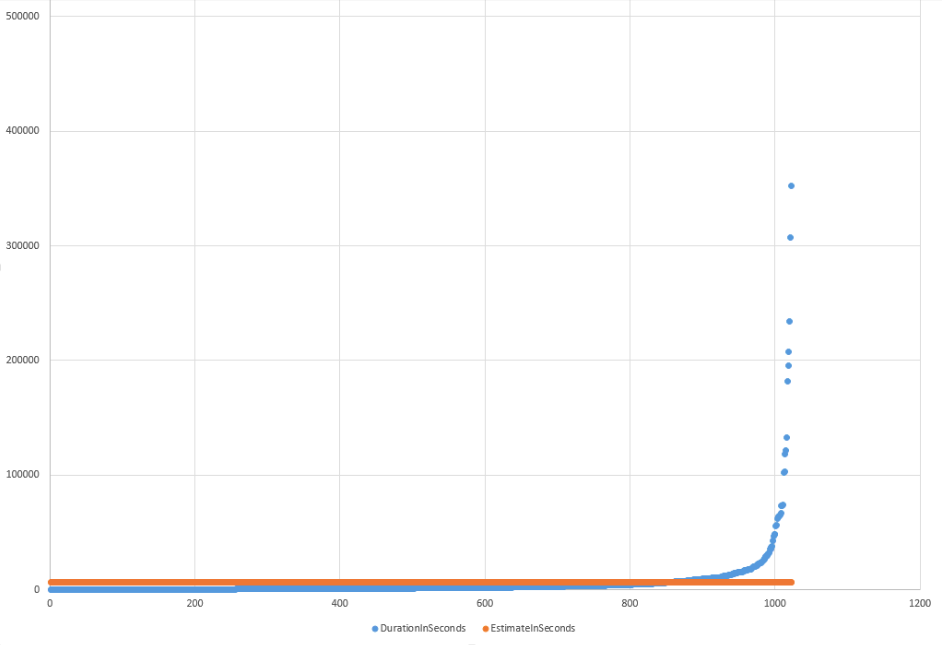
\includegraphics[width=\textwidth]{Documentation/10000-A002/a002_1-swe2020.png}
\caption{QA a002.1 - swe 2020}
\end{figure}

\textbf{on swe2021 data}

Mean squared error: 321.140.140 Percent of estimates that are too high:
85,55 \%

\begin{figure}
\centering
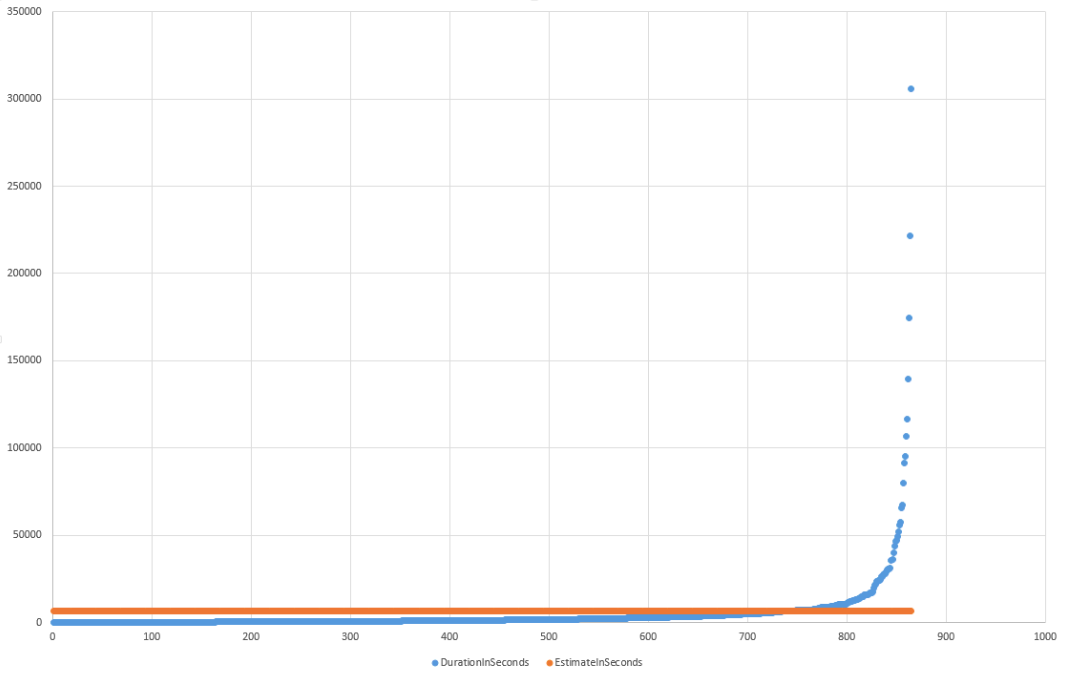
\includegraphics[width=\textwidth]{Documentation/10000-A002/a002_1-swe2021.png}
\caption{QA a002.1 - swe 2021}
\end{figure}

\hypertarget{a002.2-1}{%
\subsubsection{A002.2}\label{a002.2-1}}

\textbf{on swe2020 data}

Mean squared error: 780.036.288 Percent of estimates that are too high:
69,01 \%

\begin{figure}
\centering
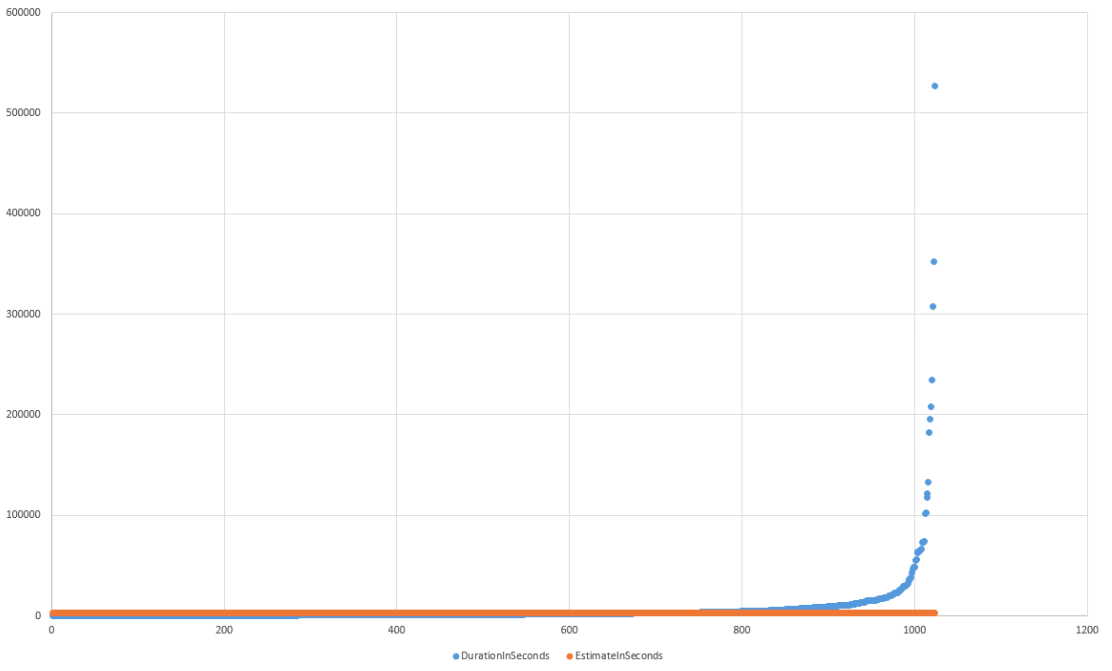
\includegraphics[width=\textwidth]{Documentation/10000-A002/a002_2-swe2020.png}
\caption{QA a002.2 - swe 2020}
\end{figure}

\textbf{on swe2021 data}

Mean squared error: 323.888.830\\
Percent of estimates that are too high: 69,94 \%

\begin{figure}
\centering
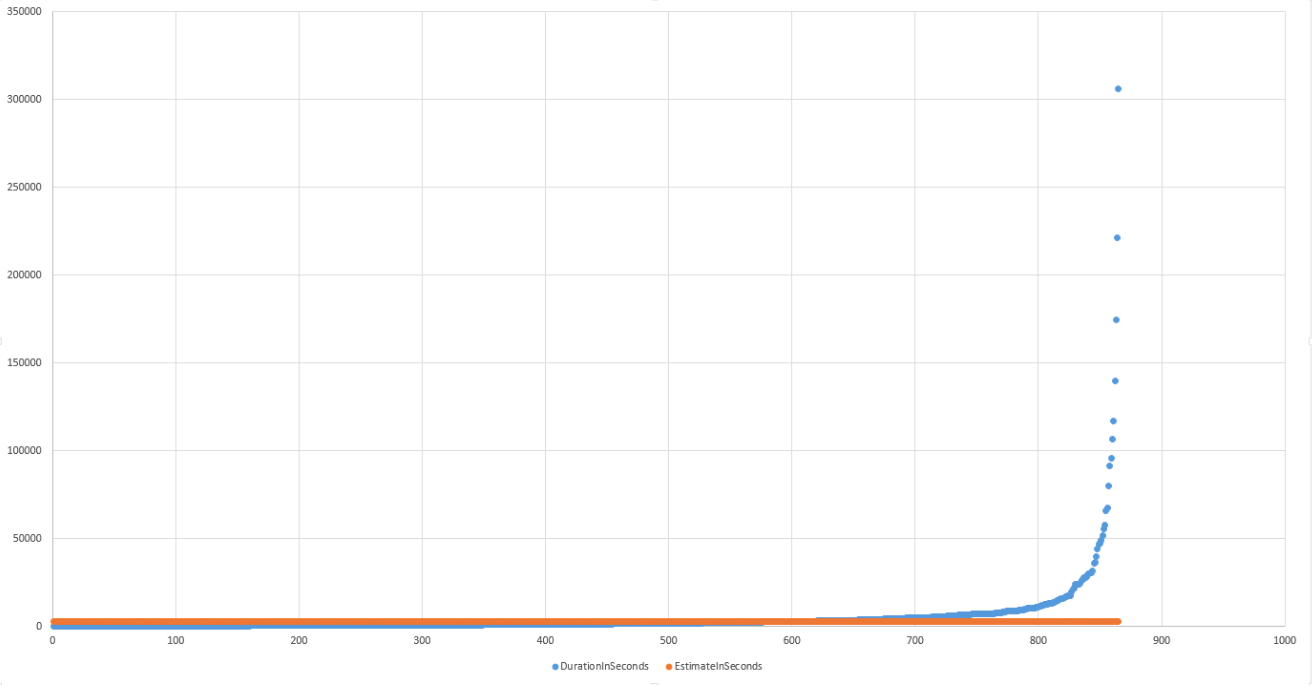
\includegraphics[width=\textwidth]{Documentation/10000-A002/a002_2-swe2021.png}
\caption{QA a002.2 - swe 2021}
\end{figure}
